\subsection{Visualizer}
Il visualizzatore è il componente che, interfacciandosi con l'utente, sincronizza gli altri moduli software e mostra i progressi dell'elaborazione in corso. Esso può operare in modalità grafica oppure testuale.

Nella modalità testuale il software si presenta come in figura \ref{fig:visualizer_textmode}, mostrando un riepilogo dei dati di configurazione e, nel caso sia stato lanciato ``in pausa'', attende che l'utente lo istruisca sul da farsi.
\begin{figure}[htp]
	\centering
	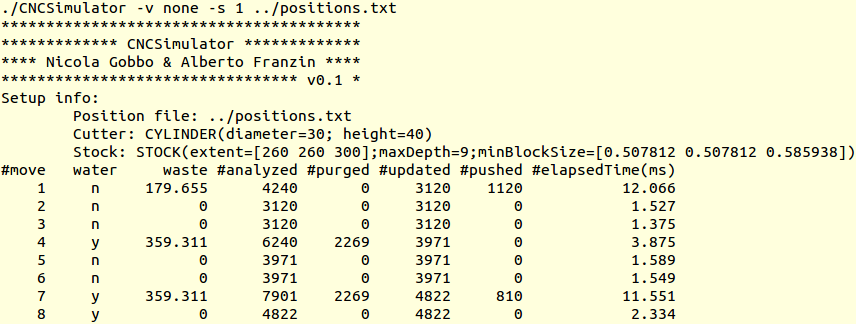
\includegraphics[width=.85\textwidth]{img/visualizer_textmode}
	\caption{\shell{CNCSimulator} avviato in modalità testuale.}
	\label{fig:visualizer_textmode}
\end{figure}

Durante l'esecuzione la modalità testuale stampa a video una nuova riga ad ogni ``mossa'' completata. Le informazioni ivi contenute riguardano il lavoro svolto dal \emph{miller} espresso in numero di foglie analizzate, aggiunte o cancellate, la quantità di materiale eroso, l'eventuale necessità di attivare il getto d'acqua e il tempo speso nell'elaborazione della mossa.

Il simulatore lanciato in modalità grafica esibisce una finestra simile a quella in figura \ref{fig:visualizer_graphicmode}. Oltre a mostrare lo stato dell'erosione in tempo reale permette all'utente di interagire con l'esecuzione in corso, mettendola in pausa, facendola avanzare di alcune mosse alla volta o disabilitando momentaneamente l'aggiornamento della scena per dedicare tutte le risorse hardware alla fresatura.
\begin{figure}[htp]
	\centering
	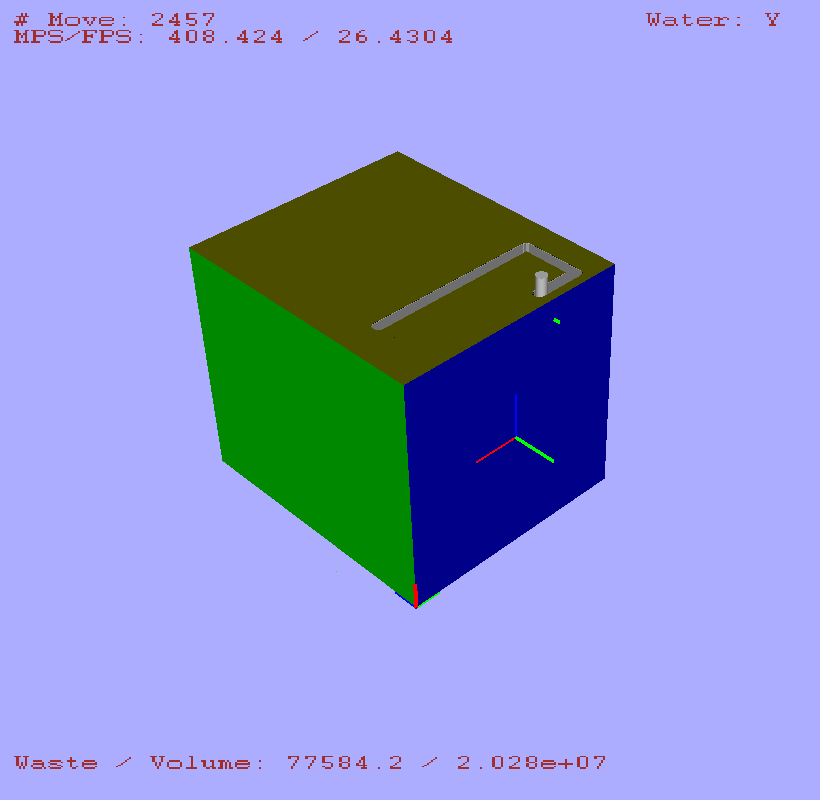
\includegraphics[width=.85\textwidth]{img/visualizer_graphicmode}
	\caption{\shell{CNCSimulator} avviato in modalità grafica.}
	\label{fig:visualizer_graphicmode}
\end{figure}

Come già detto il modulo \emph{visualizer} ha il compito di aggiornare la scena e per fare questo attende che il \emph{miller} completi almeno una mossa: questa attesa dura al più una quantità fissata di tempo, necessaria a garantire un numero di fotogrammi al secondo compreso tra 20 e 30. Nel caso in cui l'erosione venga completata in tempo, l'algoritmo procede ad aggiornare l'albero complessivo della scena richiedendo al cutter e allo stock le rispettive mesh ---che verranno quindi riposizionate in base ai parametri della mossa corrente--- e ricalcolando le varie quantità mostrate all'utente.
